%\documentclass[reponses, utf8, 11pt]{feuille}
\documentclass[utf8, 11pt]{feuille}

\newcommand{\titredutd}{\textbf{TD9 --- Le gaz sur réseau}}

\begin{document}


\begin{tcolorbox}[
        colback=gray!20,
        colframe=gray!20,
        width=\dimexpr\textwidth\relax, 
        arc=0pt,outer arc=0pt,
        ]

\texttt{Seules les calculatrices non communicantes et les notes manuscrites personnelles sont autorisées.}

\texttt{Les exercices sont totalement indépendants.}

\texttt{On notera $k_B$ la constante de Boltzmann et $h$ la constante de Planck.}

\end{tcolorbox}


Dans le modèle de gaz sur réseau, on suppose que les atomes peuvent occuper les $M$ sites d'un réseau cubique simple (de coordinence $q=6$), chaque site pouvant accueillir au plus un atome. L'interaction attractive à courte portée entre les atomes est limitée aux $q=6$ plus proches voisins et est prise en compte via l'hamiltonien :
$$
H_{gr}=-\epsilon \sum_{\langle i,j\rangle} n_i\, n_j
$$
où le taux d'occupation $n_i$ vaut $1$ si le site $i$ est occupé par un atome, $0$ s'il est vide, et où ${\langle i,j\rangle}$ indique que la somme est prise sur toutes les paires de sites plus proches voisins. La constante $\epsilon$ est positive.  Nous allons étudier ce système dans le cadre du formalisme grand-canonique à la température $T$ et au potentiel chimique $\mu$.

% ______________________________________________________________________________
\section{\medium~Le volume exclus du fluide}

On considère dans cet exercice le cas $\epsilon=0$.

\medskip

\question
En quoi ce modèle inclut-il bien l'effet de coeur dur de l'interaction atomique ?
 
\question
Que vaut la fonction de partition $Z(N,T)$ pour $N$ particules d'un tel fluide  ($N<M$)?

\question
Montrer que la grande fonction de partition $\Xi(\mu,T)$ du fluide se factorise comme le produit des grandes fonctions de partition $g$ d'un site, que l'on exprimera.

\question
Calculer la pression $P(\mu,T)$ du système ainsi que le nombre moyen $N(\mu,T)$ d'atomes. 

\question
Déterminer l'équation d'état du fluide en fonction du taux moyen d'occupation d'un site, $n=\frac{N}{M}$, puis en fonction de la densité $\rho=\frac{N}{V}$ (en introduisant $v_0=V/M$ que l'on interprétera).  Que devient cette équation dans la limite des faibles densités ?



% ______________________________________________________________________________
\section{\medium~Le fluide réel dans l'approximation de champ moyen}

On considère à présent le cas d'un fluide réel pour lequel $\epsilon>0$. On traite le problème dans l'approximation dite de champ moyen. Pour ce faire on réécrit l'hamiltonien ci-dessus en utilisant la décomposition suivante
$$
n_i n_j = (n_i -n)(n_j -n)+ n(n_i+n_j)-n^2
$$
où $n=\frac{N}{M}$ est le taux moyen d'occupation d'un site, qui est {\it indépendant} du site considéré.

\question
L'approximation de champ moyen consiste à négliger le terme de fluctuation
$$
\sum_{\langle i,j\rangle} (n_i -n)(n_j -n)
$$
Montrer que l'hamiltonien du fluide s'écrit alors comme une somme d'hamiltoniens indépendants~:
$$
H \simeq \sum_{i=1}^{M}\bigg(-6\epsilon n n_i+ 3\epsilon n^2 \bigg)
$$
Donner une interprétation du \og champ moyen\fg.

\question
Calculer la grande fonction de partition $\Xi(\mu,T,n)$ et le grand potentiel $J(\mu,T,n)$ pour $n$ {\it fixé}.

\question
Exprimer le taux moyen d'occupation d'un site sous la forme d'une équation auto-cohérente : $n=f(n)$.

\question
Montrer que l'équation d'état du fluide est donnée par~:
$$
P=-\frac{k_BT}{v_0} \ln(1-n) -\frac{3\epsilon} {v_0}n^2 =-\frac{k_BT}{v_0} \ln(1-v_0\rho) -3\epsilon v_0 \rho^2
$$
où $\rho=\frac{N}{V}$ est la densité du fluide. 

\question
Calculer le coefficient du Viriel $B_2(T)$ à partir de l'équation d'état. Son expression était-elle attendue ? Montrer que l'on retrouve le même comportement pour $B_2(T)$ que dans l'équation d'état de van der Waals.

\question
L'isotherme critique du CO$_2$ est représentée sur la figure ci-dessous. Commenter la validité de l'approximation du gaz parfait et celle du modèle de gaz sur réseau en champ moyen étudié dans cet exercice.


\begin{figure}[h!]
  \centering
  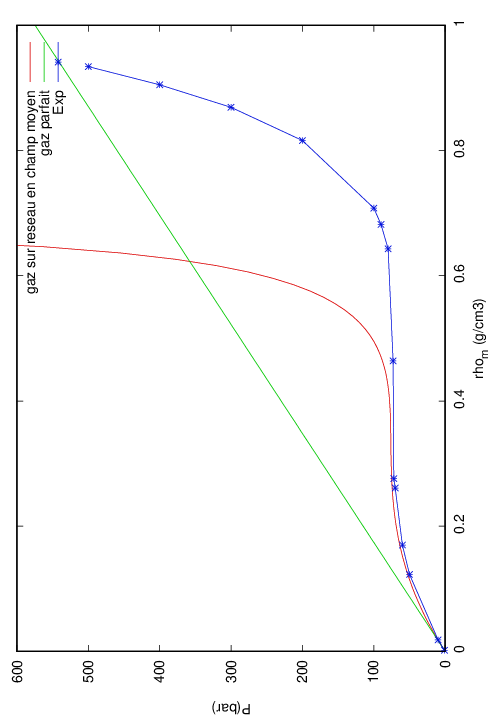
\includegraphics[scale=.7,angle=-90]{co2}
  \caption{Isotherme critique $P(\rho_m)$ du CO$_2$ à $T=T_c=304$ K
    pour le gaz parfait (ligne droite) et pour le gaz sur réseau en
    champ moyen donnée par l'équation de $H_{gr}$ (en trait
    plein), avec des valeurs ajustées de $v_0$ et de $\epsilon/k_B$. Les données expérimentales
    sont représentées par des croix. La pression est exprimée en bar
    et la masse volumique, $\rho_m$, en g.cm$^{-3}$. La masse
    volumique critique est $\rho_{m_{c}}=0,46$ g.cm$^{-3}$.}
\end{figure}


\question
Montrer que si $T$ est inférieure à une température critique $T_c$, le système peut devenir instable, c'est-à-dire que sa compressibilité isotherme
$$
\kappa =-\frac{1}{V} \frac{\partial V}{\partial P}\bigg|_T= \frac{1}{\rho} \frac{\partial \rho}{\partial P}\bigg|_T
$$
est négative pour certaines valeurs de la densité.  Déterminer les coordonnées $T_c$, $P_c$ et $\rho_c$ du point critique. Le facteur de compressibilité critique défini par $\displaystyle Z_c=\frac{P_c}{k_BT_c\rho_c}$ dépend-il du fluide considéré ? Comparer sa valeur à celle mesurée pour le CO$_2$ : $Z_c\simeq 0,27$.



\end{document}
